\chapter{Konceptgenerering} \label{Konceptgenerering}
På baggrund af problemanalysen og HoQ udarbejdes en række konceptuelle løsninger, der vurderes med udgangspunkt i de krav, der er specificeret i afsnit \ref{Endelige kravspecifikationer}. Indledningsvis identificeres de enkelte funktioner og delfunktioner, som en robot til fremstilling af speckle patterns skal udføre. Herefter udarbejdes delløsninger for hver delfunktion gennem en systematisk morfologisk analyse, hvorefter de enkelte delløsninger integreres til samlede konceptforslag. 
\section{Funktioner} \label{Funktioner}
Funktioner defineres som en opgave der skal udføres, og kan yderligere opdeles i delfunktioner (\cite{Ullman2018TheProcess}). Opgaverne der skal udføres i forbindelse med fremstilling af speckle pattern med en robot, illustreres i et flowchart, se figur \ref{fig: flowchart}. Figuren aflæses ved at følge pilene fra en handling til en anden, fra start til slut. 

\begin{figure}[H]
    \centering
    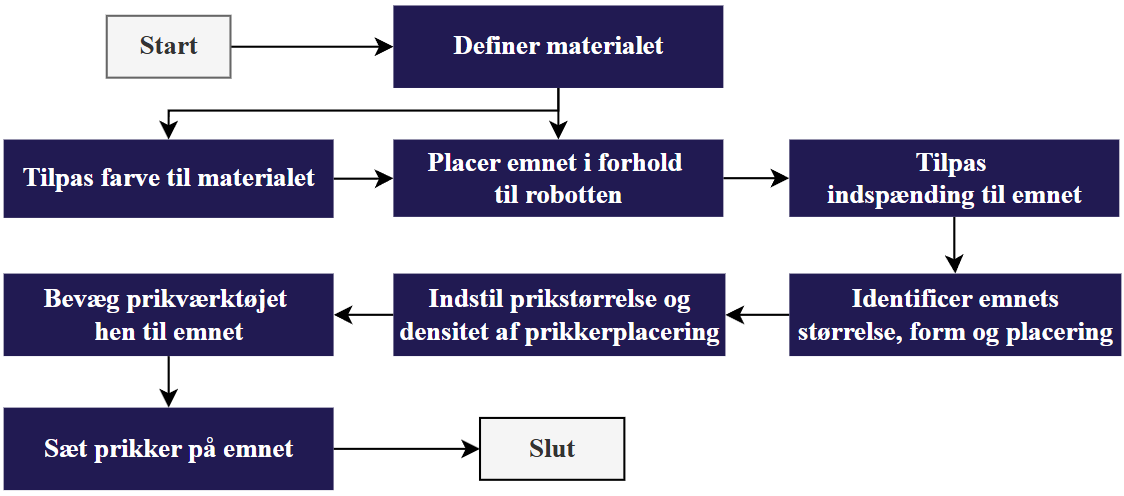
\includegraphics[width=1\linewidth]{Sections/5 Konceptgenerering/Media/Flowchart.png}
    \caption{Flowchart for en robot der skal påsætte speckle patterns}
    \label{fig: flowchart}
\end{figure} \plainbreak{-0.5}

Flowchartet i figur \ref{fig: flowchart} benyttes til at identificere de funktioner og delfunktioner, der ses i figur \ref{Figur: Funktionstræ}. Det er valgt, at opstille alle funktioner i et funktionstræ, for at danne et klart overblik over funktioner og delfunktioner en robot, der sætter speckle patterns skal udføre. Disse benyttes efterfølgende i en morfologisk analyse.  


\newpage
\begin{figure}[H]
\centering
\begin{tikzpicture}
[
    graybox/.style={rectangle, fill=lightgray!20, 
        minimum width=6cm, minimum height=0.8cm, align=center},
    box/.style={rectangle, fill=aaublue, text=white, 
        minimum width=6cm, minimum height=0.8cm, align=center},
    tallbox/.style={rectangle, fill=aaublue, text=white, 
        minimum width=5.8cm, minimum height=1.8cm, align=center, text width=5.8cm},
    arrow/.style={-Stealth, thick}]

% Problemanalyse
\node[tallbox, rotate = 90] (funktioner) {\Large \textbf{Robot til fremstilling af speckle patterns}};

% Funktioner
\node[box, right=1.cm of funktioner.south east, anchor=north west] (bevaegelse) {\textbf{Bevægelse}};
\node[box, below=.8cm of bevaegelse] (kontrolsystem) {\textbf{Kontrolsystem}};
\node[box, below=.8cm of kontrolsystem] (saette) {\textbf{Sætte prikker}};
\node[box, below=.8cm of saette] (fastholde) {\textbf{Fastholde emne}};


%beskrivele Funktion
\node[graybox, above=.2cm of bevaegelse](Funktion){\textbf{Funktioner}};
\draw[lightgray!40, very thick] (1.8,3.1) rectangle (8,-3.2);

%beskrivele delfunktion
\node[graybox, right=1.cm of Funktion](Delfunktion){\textbf{Delfunktioner}};
\draw[lightgray!40, very thick] (8.8,3.1) rectangle (15,-3.2);


% Delfunktioner til Kontrolsystem
\node[box, below=1.3cm of Delfunktion] (brugerflade) {\textbf{Brugerflade}};
\node[box, below=.2cm of brugerflade] (formanalyse) {\textbf{Kalibrering af emne placering}};

% Delfunktioner til Fastholdelse
\node[box, below=1.4cm of formanalyse] (indspaend) {\textbf{Indspænding}};
\node[box, below=.2cm of indspaend] (understot) {\textbf{Understøttelse}};


% Pile
\draw[arrow] (funktioner.south) -- ++(0.5,0) |- (bevaegelse);
\draw[arrow] (funktioner.south) -- ++(0.5,0) |- (saette);
\draw[arrow] (funktioner.south) -- ++(0.5,0) |- (kontrolsystem);
\draw[arrow] (funktioner.south) -- ++(0.5,0) |- (fastholde);

\draw[arrow] (kontrolsystem.east) -- ++(0.5,0) |- (brugerflade);
\draw[arrow] (kontrolsystem.east) -- ++(0.5,0) |- (formanalyse);

\draw[arrow] (fastholde.east) -- ++(0.5,0) |- (indspaend);
\draw[arrow] (fastholde.east) -- ++(0.5,0) |- (understot);

\end{tikzpicture}
\caption{Funktionstræ}
\label{Figur: Funktionstræ}
\end{figure} \plainbreak{-0.5}

Det er valgt ikke at medtage 'tilpas farve til materialet' da der er afgrænset fra farvemidlet i afsnit \ref{Afgrænsning}.


\subsubsection{Bevægelse} \plainbreak{-0.5}
Metode til at flytte prikværktøjet og/eller emnet i forhold til hinanden, der muliggør fremstillingen af et speckle pattern på et 2D plan.



\subsubsection{Kontrolsystem}\plainbreak{-0.5}
%Kontrolsystemet bestemmer hvor og hvornår der skal sættes prikker, og giver feedback til brugeren. Dette er nødvendigt for, at robotten kan påsætte det ønskede speckle pattern, samt give brugeren mulighed for at kunne starte og stoppe maskinen. Kontrolsystemet har to delfunktioner; brugerflade, som skal modtage input og give feedback tilbage til brugeren der betjener robotten og Kalibrering af emnets placering. Kalibreringen er til for, at robotten ved hvor emnet er placeret, dets størrelse og form. For at undgå påsætning af speckle patterns udenfor emnet, er det nødvendig med identifikation af emnets dimensioner.

Det er i afsnit \ref{Afgrænsning} valgt, at afgrænse fra elektronik og software, hvorfor kontrolsystemet ikke medtages i den morfologiske analyse. Det fysiske design af kontrolsystemet har betydning for designet af de mekaniske dele, hvorfor delkoncepter til kontrolsystemet er overfladisk undersøgt i bilag \ref{Bilag - morf til kontrolsystem}.



\subsubsection{Sætte prikker} \plainbreak{-0.5}
En essentiel del af robottens funktion er, at den sætter speckle patterns. Delfunktioner til at sætte prikker vurderes at være så afhængige at hvilken overordnet metode til at sætte prikker der bliver, og kan derfor ikke yderligere specificeres, før den overornede metode er valgt. Dette er fordi løsningerne fra problemanalysens afsnit \ref{DIC afsnit}, har stor variation i metoden til at påsætte prikker og de delfunktioner de kræver. 



\subsubsection{Fastholde emnet} \plainbreak{-0.5}
Emnet skal fastholdes, så emnet ikke flyttes under påsætning af speckle pattern. Fastholdelsen er opdelt i indspænding og understøtning. Emnet må maksimalt flyttes \(\SI{0,01}{mm}\) under påføring af speckle patterns, hvilket nødvendiggør indspænding af emnet, så der ikke sker flytning. Understøtningen defineres som den overflade emnet kan placeres på, hvorefter det kan fastgøres af indspændingen. Understøtningen har til formål at understøtte emnet fra kræfter som tyngdekraften, for at indspændingen kan være så simpel som muligt. 


%Delfunktionerne til kontrolsystem vurderes at være af minimal betydning for vægtningen af konceptforslagene og afhænger af hvilke mekaniske koncepter der vælges. Der laves derfor først en morfologisk analyse af de mekaniske dele, der omfatter; bevægelse, priksætning, indspænding og understøttelse, efterfulgt af en morfologisk analyse af kontrolsystemet.   

 

\plainbreak{2}
\section{Morfologisk analyse af mekaniske dele} \label{Morfologisk analyse - mekaniske dele}
Alle delfunktioner, der omhandler mekaniske dele beskrevet i afsnit \ref{Funktioner}, opsættes i en morfologisk analyse, hvor delløsninger til hver enkelt delfunktion benyttes til at danne samlede løsningskoncepter. Koncepterne skal overholde alle de ufravigelige krav opsat i afsnit \ref{Endelige kravspecifikationer}, for at blive medtaget i den morfologiske analyse.

Antallet af kombinationer af delløsninger, er vurderet for stor til at alle koncepter har kunne gennemgås. Der er fravalgt delløsninger, på baggrund af mangel på effektivitet og nøjagtighed. Der er udvalgt ni koncepter der arbejdes videre med, disse koncepter kan ses i tabel \ref{tab: morfologisk analyse af mekanikse}. Konceptforslagene fra den morfologiske analyse, kan findes ved at følge de forskellige farver/former, der hver repræsenterer et koncept skabt af delkoncepter.


%en farve/form hvert element i det bestemte koncept. Ved at følge for eksempel den lilla cirkel ($\lillacirc$), findes alle delkoncepterne som koncept 1 består af.

%Antallet af kombinationer af delløsninger, har resulteret i en mængde af koncepter vurderet for stor til at alle koncepter har kunne gennemgås

\begin{table}[H]
   \caption{Morfologisk analyse. 1 $=$ \protect\lillacirc, 2 $=$ \protect\bluebox, 3 $=$ \protect\cyanbox, 4 $=$ \protect\blueangle, 5 $=$ \protect\greenangle, 6 $=$ \protect\gulangle, 7 $=$ \protect\orangeangle, 8 $=$ \protect\pinkstar og 9 $=$ \protect\redkant}
    \centering
    \begin{tabular}{|l|p{3.1cm}|p{3.1cm}|p{3.1cm}|p{3.1cm}|} \cline{2-5}      
           \multicolumn{1}{l|}{} & \multicolumn{4}{|c|}{\cellcolor{aaublue} \textcolor{white}{\textbf{Delkoncepter til mekaniske delfunktioner }}} \\ \cline{2-5} \multicolumn{1}{l|}{}  & \multicolumn{1}{c|}{ \cellcolor{lightgray!20} \textbf{1}} & \multicolumn{1}{|c|}{\cellcolor{lightgray!20} \textbf{2}} & \multicolumn{1}{c|}{\cellcolor{lightgray!20} \textbf{3}} & \multicolumn{1}{c|}{\cellcolor{lightgray!20} \textbf{4}}  \\ \cline{2-5} \specialrule{0pt}{0.5pt}{0pt}
          
        %Bevægelse
        \rotatebox[origin=c]{90}{\cellcolor{aaublue} \textcolor{white}{\textbf{Bevægelse }}} & \makecell{\small Lineær bevægelse  \\ \includegraphics[width=0.98\linewidth]{Sections/5 Konceptgenerering/Media/lineær.png} \\ \lillacirc \ \bluebox \ \orangeangle \ \redkant} & \makecell{\small Robotarm \\ 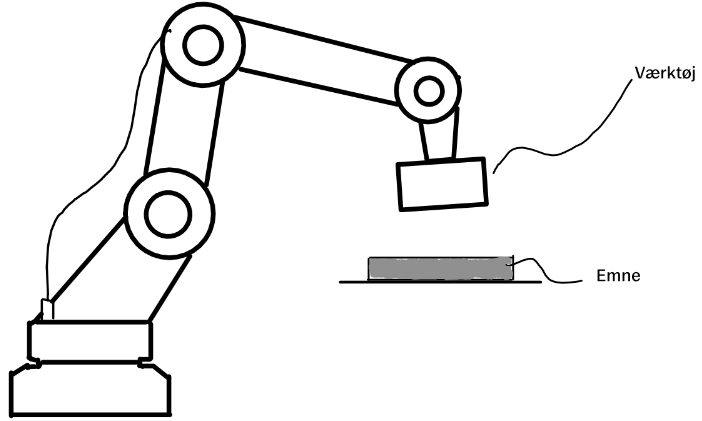
\includegraphics[width=0.98\linewidth]{Sections/5 Konceptgenerering/Media/arm.png} \\ \gulangle} & \makecell{\small Deltarobot\\ 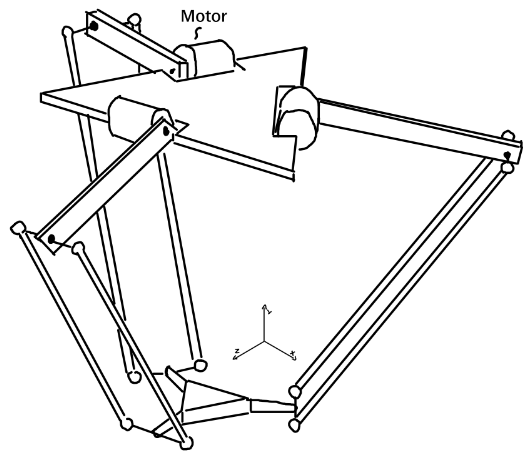
\includegraphics[width=0.98\linewidth]{Sections/5 Konceptgenerering/Media/delta.png} \\ \cyanbox \ \blueangle \ \pinkstar } & \makecell{\small Drejeskive \\ 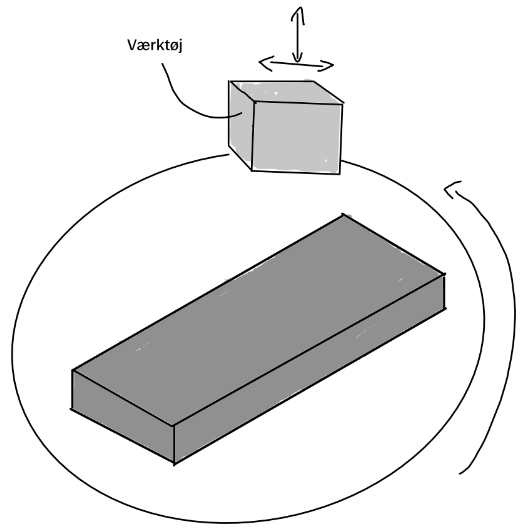
\includegraphics[width=0.98\linewidth]{Sections/5 Konceptgenerering/Media/Drejeskive.png} \\ \greenangle}\\  \specialrule{1pt}{0pt}{0pt}


        %Sæt prik
        \rotatebox[origin=c]{90}{\cellcolor{aaublue} \textcolor{white}{\textbf{\small Sætte prikker}}} & \makecell{\small Sætte dråbe \\ \includegraphics[width=0.8\linewidth]{Sections/5 Konceptgenerering/Media/åbnelukke.png} \\ \lillacirc \ \bluebox \ \cyanbox \ \blueangle \ \greenangle }& \makecell{ \small Spids røre  \\ emnet \\ \includegraphics[width=0.2\linewidth]{Sections/5 Konceptgenerering/Media/spids røre.png} \\ \gulangle \ \orangeangle \ \pinkstar \ \redkant} & \makecell{\small Spray \\ 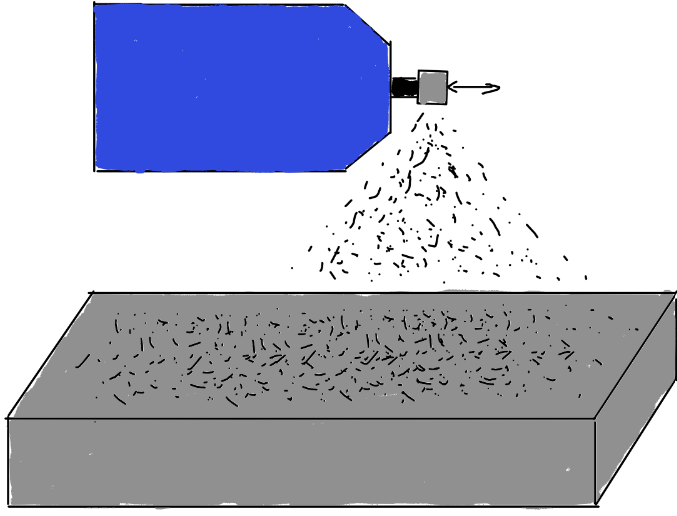
\includegraphics[width=0.8\linewidth]{Sections/5 Konceptgenerering/Media/spray.png}} & \makecell{\small Stempel \\ 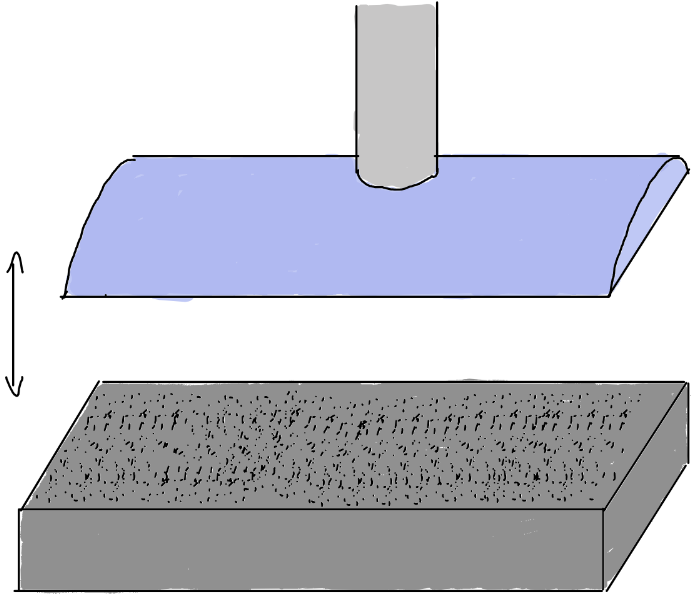
\includegraphics[width=0.98\linewidth]{Sections/5 Konceptgenerering/Media/stempel.png}}  \\ \specialrule{1pt}{0pt}{0pt}

        %Indspænding
        \rotatebox[origin=c]{90}{\cellcolor{aaublue} \textcolor{white}{\textbf{Indspænding}}} & \makecell{\small Press på emnet \\ \includegraphics[width=0.7\linewidth]{Sections/5 Konceptgenerering/Media/Press på emnet.png} \\ \bluebox \ \orangeangle \ \gulangle}  & \makecell{Sug \\ 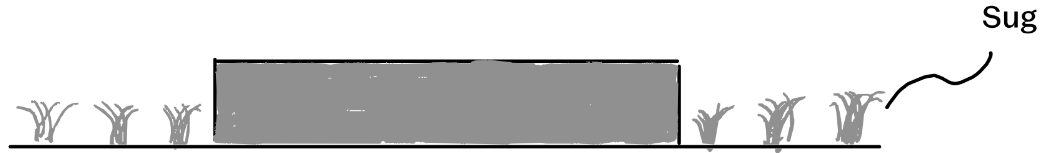
\includegraphics[width=0.98\linewidth]{Sections/5 Konceptgenerering/Media/sug.png} \\ \lillacirc \ \redkant} & \makecell{\small Vakuumpose\\ med fyld \\ 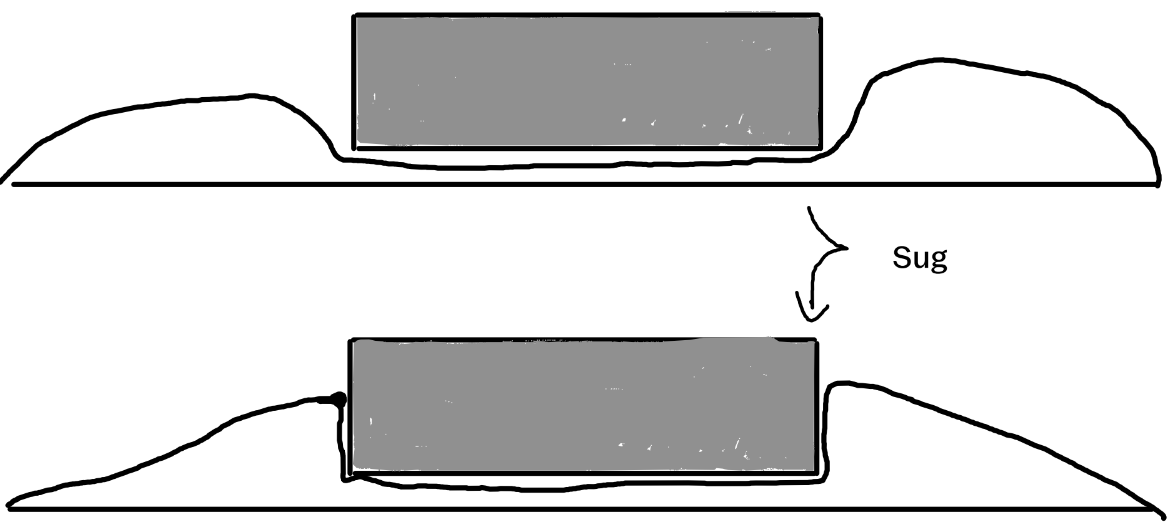
\includegraphics[width=0.98\linewidth]{Sections/5 Konceptgenerering/Media/vakuum.png} \\ \cyanbox \ \greenangle \ \pinkstar}&  \makecell{\small Ru overflade \\ 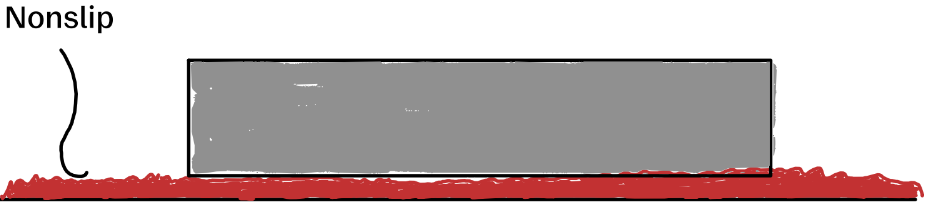
\includegraphics[width=0.98\linewidth]{Sections/5 Konceptgenerering/Media/rug.png} \\ \blueangle}  \\ \specialrule{1pt}{0pt}{0pt}

        %Understøttelse
        \rotatebox[origin=c]{90}{\cellcolor{aaublue} \textcolor{white}{\textbf{Understøttelse}}} & \makecell{\small Plade \\ under emnet \\ \includegraphics[width=0.98\linewidth]{Sections/5 Konceptgenerering/Media/Understøttelse plade.png} \\ \lillacirc \ \cyanbox \ \blueangle \ \greenangle \\ \orangeangle  \gulangle \ \pinkstar \  \redkant } & \makecell{\small Understøttet \\ i punkter \\ \includegraphics[width=0.9\linewidth]{Sections/5 Konceptgenerering/Media/Understøttelse i punkter.png} \\ \bluebox} & &    \\ \hline
        
    \end{tabular}
    \label{tab: morfologisk analyse af mekanikse}
\end{table} \plainbreak{-0.5}

I denne morfologiske analyse, er der set bort fra delløsninger med spray og stempel, se tabel \ref{tab: morfologisk analyse af mekanikse}. Dette er gjort, da der ikke kan findes koncepter med disse delløsninger, som kan skille sig ud og konkurrere på de vilkår der ønskes. Spraymetoden opnår ikke den pålidelighed i prikpræcision, der ønskes for produktet, hvilket er et essentielt punkt, for at produktet vil være konkurrencedygtigt på markedet. Stemplet kan opnå en tilstræklig præcision, i stedet vil det ikke være en tilstrækkelig fordel, da det ikke er nødvendigt med en maskine til at stemple en overflade. Da det er et krav, at der skal laves en robot, giver det ikke mening, at gå videre med den delløsning. Robotarmen og drejeskiven anvendes få gange da det vurderes at deres kompleksitet ikke opvejes med markante fordele. De bliver alligevel inkluderet i et par koncepter, for ikke at gå klip af eventuelle gode løsninger.

Indspændingsdelløsningerne kan også sætte krav til understøtningen. Et eksempel er, at det ikke er muligt at lave sug-funktionen eller vakuumposen med fyld, med en understøttelse i punkter. Dette har medført, at en større andel af koncepterne gør brug af understøtning i form af en plade, frem for understøttelse i punkter. 





\subsection{Konceptforslag til mekaniske dele} \label{Konceptforlag - mekaniske dele}

\begin{figure}[H]
    \centering
    \begin{subfigure}[b]{0.34\textwidth}
        %centering
        \includegraphics[width=\textwidth]
        {Sections/5 Konceptgenerering/Media/1.Løsning.png}
        \caption{Konceptforslag 1 \protect\lillacirc}
        \label{fig:Konceptforslag 1}
    \end{subfigure}
    \begin{subfigure}[b]{0.32\textwidth}
        %centering
        \includegraphics[width=\textwidth]
        {Sections/5 Konceptgenerering/Media/2.Løsning.png}
        \caption{Konceptforslag 2 \protect\bluebox}
        \label{fig:Konceptforslag 2}
    \end{subfigure}
    \begin{subfigure}[b]{0.24\textwidth}
        %centering
        \includegraphics[width=\textwidth]
        {Sections/5 Konceptgenerering/Media/3.Løsning.png}
        \caption{Konceptforslag 3 \protect\cyanbox}
        \label{fig:Konceptforslag 3}
    \end{subfigure}
    \caption{Konceptforslag 1 til 3}
\end{figure} \plainbreak{-0.5}

\textbf{Konceptforslag 1  \protect\lillacirc}  bevæger sig lineært i tre dimensioner og benytter sig af en mekanisme der afsætter dråber, som tager udgangspunkt i en inkjet. Til at fastholde emnet, som skal prikkes, fastspændes det ved brug af sug. Her vil der skabes undertryk under emnet, som vil resultere i at emnet er fastspændt. Sammen med sug vil emnet understøttes af en fast plade under emnet.

\textbf{Konceptforslag 2 \protect\bluebox} 
bevæger sig på samme måde som koncept 1. Koncept 2 bruger som koncept 1 også dråbemekanismen. Denne iteration er unik i fastholdelsen, hvor der bruges pres på emnet fra siderne af, til at holde emnet fast. Her er, fremfor understøttelse i en plade, understøttelse i punkter, som er hvor emnet skal stabiliseres over flere kontaktpunkter.


\textbf{Konceptforslag 3 \protect\cyanbox} 
har sin bevægelse igennem en deltarobot, som trækker i sine arme for at flytte på hovedet over prikfladen. Der gøres også brug af mekanisme der afsætter dråber. Indspændingen laves ved at have en vakuumpose der er fyldt med små kugler, som bliver låst i position efter luften tages ud af posen. Hvis prikobjektet placeres på posen, vil de små kugler position låse objektets position. Dette koncept gør brug af pladen under emnet, som understøtning.

\begin{figure}[H]
    \centering
    \begin{subfigure}[b]{0.27\textwidth}
        %centering
        \includegraphics[width=\textwidth]
        {Sections/5 Konceptgenerering/Media/4.Løsning.png}
        \caption{Konceptforslag 4 \protect\blueangle}
        \label{fig:Konceptforslag 4}
    \end{subfigure}
    \begin{subfigure}[b]{0.28\textwidth}
        %centering
        \includegraphics[width=\textwidth]
        {Sections/5 Konceptgenerering/Media/5.Løsning.png}
        \caption{Konceptforslag 5 \protect\greenangle}
        \label{fig:Konceptforslag 5}
    \end{subfigure}
    \begin{subfigure}[b]{0.35\textwidth}
        %centering
        \includegraphics[width=\textwidth]
        {Sections/5 Konceptgenerering/Media/6.Løsning.png}
        \caption{Konceptforslag 6 \protect\gulangle}
        \label{fig:Konceptforslag 6}
    \end{subfigure}
    \caption{Konceptforslag 4 til 6}
\end{figure} \plainbreak{-0.5}

\textbf{Konceptforslag 4 \protect\blueangle} 
bevæger sig med udgangspunkt i en deltarobot, ligesom koncept 3. Koncept 4 gør brug af mekanismen der sætter dråber. Emnet vil ligge på en rug overflade, så emnet ikke bevæger sig. Derudover vil emnet blive understøttet af en plade under emnet.


\textbf{Konceptforslag 5 \protect\greenangle} 
placerer emnet på en drejeskive, så prikværktøjet kun skal bevæge sig fra side til side (x-retningen), op og ned (z-aksen) og rotere emnet om z-aksen. Prikværktøjet benytter mekanismen der afsætter dråber prikplacering. Emnet indspændes igennem posen med kugler, der sættes i vakuum og låser emnet. Emnet er understøttet af en plade.


\textbf{Konceptforslag 6 \protect\gulangle} 
bruger en flerleddet robotarm til sine bevægelser, som gør rotationer i led til en kontrolleret bevægelse til prikplacering. I dette koncept gøres der brug af tuschmetoden, som indebærer at føre et farvefyldt emne ned og berøre prikfladen, for at overføre farven. Konceptet gør brug af indspænding fra siden, og gør også brug af en plade under emnet til understøtning.

\begin{figure}[H]
    \centering
    \begin{subfigure}[b]{0.3\textwidth}
        %centering
        \includegraphics[width=\textwidth]
        {Sections/5 Konceptgenerering/Media/7.Løsning.png}
        \caption{Konceptforslag 7 \protect\orangeangle}
        \label{fig:Konceptforslag 7}
    \end{subfigure}
    \begin{subfigure}[b]{0.3\textwidth}
        %centering
        \includegraphics[width=\textwidth]
        {Sections/5 Konceptgenerering/Media/8.Løsning.png}
        \caption{Konceptforslag 8 \protect\pinkstar}
        \label{fig:Konceptforslag 8}
    \end{subfigure}
    \begin{subfigure}[b]{0.3\textwidth}
        %centering
        \includegraphics[width=\textwidth]
        {Sections/5 Konceptgenerering/Media/9.Løsning.png}
        \caption{Konceptforslag 9 \protect\redkant}
        \label{fig:Konceptforslag 9}
    \end{subfigure}
    \caption{Konceptforslag 7 til 9}
\end{figure} \plainbreak{-0.5}

\textbf{Konceptforslag 7 \protect\orangeangle} 
benytter en lineær bevægelse til bevægelse af prikværktøjet. Prikmetoden er som koncept 6 tuschmetoden. Der gøres her brug af en indspænding fra siderne. Der bruges en plade under emnet til at understøtte emnet.


\textbf{Konceptforslag 8 \protect\pinkstar}
bevæger sig i form af en deltarobots armjustering. Konceptet skal sætte prikker med tuschmetoden som koncept 6 og 7. Indspændingen kommer af vakuumpose med fyld, der låser emnets placering. Der bruges også her en plade under emnet til understøttelse.


\textbf{Konceptforslag 9 \protect\redkant} 
bevæger sig lineært i tre retninger for at justere prikværktøjet, samt benytter en prik metode, som en tusch. Emnet indspændes ved at danne et undertryk under emnet ved brug af sug, samt bliver understøttet af en plade under emnet.


 
\plainbreak{2}
\subsection{Koncept screening af mekaniske dele} \label{Mekanisk system - vurdering}
%- Tush er mere præcis i prikstørrelse end åbne/lukke \\
%- Delta robot hurtigere end lineær bevægelse \\
For at finde frem til et endeligt løsningskoncept for de mekaniske dele, vurderes de ni udvalgte koncepter igennem en screening. De udvalgte koncepter vurderes ud for et sæt af kriterier, som kan ses i tabel \ref{tab:selektionsskema mekanisk}. Alle delløsninger, som koncepterne består af, er blevet vurderet i forhold til kriterierne (se bilag \ref{Bilag mekaniske delkonceptervurdering}), hvortil de samlede værdier af et koncepts delløsninger, er lig konceptets samlede vurdering. Vurderingerne er sket ved at sætte koncept 1's (\lillacirc) delløsninger som en standard/reference, og dertil vurdere de andre delløsninger, i forhold til koncept 1. Hvert kriterie er tildelt en vægt, som sikrer vigtigere kriterier har større betydning for udfaldet. Vægtene er fremsat på baggrund af vægtningerne fra kapitel \ref{Trin 1-4}, tabel \ref{tab: trin 1 til 4}, og designspecifikationer fra HoQ i kapitel \ref{Kravspecifikation}.

\renewcommand{\arraystretch}{1.6}
\begin{table}[H]
    \centering
    \footnotesize
    \caption{Screening skema. Værdierne er summen af delkoncepternes vurdering som ses i bilag \ref{Bilag mekaniske delkonceptervurdering}.}
    \begin{tabular}{|l|c||c c c c c c c c||r|} \cline{2-10}

        \multicolumn{1}{c}{}& \multicolumn{9}{|c|}{\cellcolor{aaublue} \textcolor{white}{\textbf{Konceptforslag til mekaniske dele}}} \\ \hline
         
        \multicolumn{1}{|c}{\cellcolor{lightgray!20}\textbf{Vurderingskriterier}} & \multicolumn{1}{|c||}{\cellcolor{lightgray!20}\textbf{1 \protect\lillacirc}}  &\multicolumn{1}{c}{\cellcolor{lightgray!20}\textbf{2 \protect\bluebox}} &\multicolumn{1}{c}{\cellcolor{lightgray!20}\textbf{3 \protect\cyanbox}} &\multicolumn{1}{c}{\cellcolor{lightgray!20}\textbf{4 \protect\blueangle}} &\multicolumn{1}{c}{\cellcolor{lightgray!20}\textbf{5 \protect\greenangle}} &\multicolumn{1}{c}{\cellcolor{lightgray!20}\textbf{6 \protect\gulangle}}   &\multicolumn{1}{c}{\cellcolor{lightgray!20}\textbf{7 \protect\orangeangle}} &\multicolumn{1}{c}{\cellcolor{lightgray!20}\textbf{8 \protect\pinkstar}} &\multicolumn{1}{c||}{\cellcolor{lightgray!20}\textbf{9 \protect\redkant}} &\multicolumn{1}{r|}{\cellcolor{lightgray!20}\textbf{Vægt}} \\ \hline
         
    %% Vurdering
        % Præcision af prik størrelse
         \multicolumn{1}{|l|}{\cellcolor{aaublue} \textcolor{white}{\textbf{Præcision af prik størrelse}}} 
         & 0 & 0 & 0 & 0 & 0 & -1 & -1 & -1 & -1 & 3\\ \hline
        % Præcision af prik placering  
         \multicolumn{1}{|l|}{\cellcolor{aaublue} \textcolor{white}{\textbf{Præcision af prik placering}}} 
         & 0 & 0 & -1 & -1 & -1 & 1 & 1 & 0 & 1 & 3 \\ \hline
        % Fastholdelse
         \multicolumn{1}{|l|}{\cellcolor{aaublue} \textcolor{white}{\textbf{Fastholdelse}}} 
         & 0 & 0 & 1 & -3 & 0 & 1 & 1 & 1 & 0 & 5  \\\hline
        % Hurtighed
         \multicolumn{1}{|l|}{\cellcolor{aaublue} \textcolor{white}{\textbf{Hurtighed}}} 
         & 0 & 0 & 0 & 2 & -2 & -2 & -1 & -1 & -1 & 2 \\\hline
        % Brugerinvolvering
         \multicolumn{1}{|l|}{\cellcolor{aaublue} \textcolor{white}{\textbf{Brugerinvolvering}}} 
         & 0 & -2 & 0 & 0 & 0 & -1 & -1 & 0 & 0 & 2 \\\hline
        % Holdbarhed
         \multicolumn{1}{|l|}{\cellcolor{aaublue} \textcolor{white}{\textbf{Holdbarhed}}} 
         & 0 & 1 & 0 & 1 & 0 & -1 & 0 & -1 & -1 & 1 \\\hline
        % Kompleksitet ved fremstilling
         \multicolumn{1}{|l|}{\cellcolor{aaublue} \textcolor{white}{\textbf{Kompleksitet ved fremstilling}}} 
         & 0 & 1 & -1 & 1 & 0 & 1 & 2 & 0 & 1 & 1 \\\hline
        % Kompleksitet ved samling
        \multicolumn{1}{|l|}{\cellcolor{aaublue} \textcolor{white}{\textbf{Kompleksitet ved samling}}} 
        & 0 & -1 & 0 & 1 & 0 & -1 & 0 & 1 & 1 & 1 \\ \hline \specialrule{0pt}{2pt}{0pt} \cline{1-10}
%% Samlet score og rank
         \multicolumn{1}{|r|}{\cellcolor{lightgray!10} \textbf{Vægtet score}}& 0 & -3 & 1 & -11 & -7 & -2 & 3 & 0 & \multicolumn{1}{c|}{-1}  & \multicolumn{1}{c}{} \\\cline{1-10} 

         \multicolumn{1}{|r|}{\cellcolor{lightgray!10}\textbf{Rangering}}& 3 & 7 & \multicolumn{1}{c}{\cellcolor{OliveGreen}\textbf{2}} & 9 & 8 & 6 &  \multicolumn{1}{c}{\cellcolor{OliveGreen}\textbf{1}} & 3 & \multicolumn{1}{c|}{5}  & \multicolumn{1}{c}{} \\\cline{1-10}
    \end{tabular}
    \label{tab:selektionsskema mekanisk}
\end{table} \plainbreak{-0.5}

Ud fra screeningen blev koncept 3 (\cyanbox) og 7 (\orangeangle) vurderet til at være de to bedste kandidater. De to konceptforslags forskellige delløsninger blev sammenlignet, for at undersøge om en kombination, af de to eventuelt kunne skabe et bedre koncept. Det resulterede i, at koncept 7 i kombination med koncept 3's sæt prik delløsning, vil øge præcisionen og derved danne det bedste koncept. Det sammensatte koncept 10 ($\protect\mathcolor{BrickRed}{\clubsuit}$) (bilag \ref{Bilag mekaniske delkonceptervurdering}) får 4 point i den vægtede score, hvilket er 1 point mere end konceptforslag 7. Screeningsskemaet for det endelige koncept kan ses i bilag \ref{Bilag mekaniske delkonceptervurdering}. 



\begin{comment}
\begin{table}[H]
    \caption{}
    \centering
    \begin{tabular}{|c|c|c|c|} 
        \hline
        \multicolumn{4}{|c|}{\cellcolor{aaublue} \textcolor{white}{\textbf{Endelig mekanisk koncept }}} \\ \hline
        \rowcolor{lightgray!10} Bevægelse & Sætte prikker& Indspænding & Understøttelse \\ \hline
        \multicolumn{1}{|p{3.4cm}|}{
        \includegraphics[width=0.80\linewidth]{Sections/5 Konceptgenerering/Media/lineær.png}} &  
        \multicolumn{1}{p{3.4cm}|}{\includegraphics[width=0.80\linewidth]{Sections/5 Konceptgenerering/Media/åbnelukke.png}} &
        \multicolumn{1}{p{3.4cm}|}{\includegraphics[width=0.80\linewidth]{Sections/5 Konceptgenerering/Media/Press på emnet.png}} &
        \multicolumn{1}{p{3.4cm}|}{ \includegraphics[width=0.80\linewidth]{Sections/5 Konceptgenerering/Media/Understøttelse plade.png}} \\ \hline
    \end{tabular}
    \label{tab: endeligkonceptmekanisk}
\end{table}
\end{comment}



\begin{comment}
\begin{table}[H]
    \centering
    \caption{Selektion skema, hvor 0 = neutral, + = bedre end og - = værre end.  Den samlet score er beregnet ved "Sam af +" + "Sum af -"}
    \begin{tabular}{|>{\columncolor{lightgray!20}}c|c|c|*{1}{>{\centering\arraybackslash}p{.4cm}} || *{8}{>{\centering\arraybackslash}p{.4cm}|}} \cline{4-12}

        \multicolumn{3}{c}{}& \multicolumn{9}{|c|}{\cellcolor{aaublue} \textcolor{white}{\textbf{Konceptforslag til mekaniske dele}}} \\ \cline{4-12}
         
        \multicolumn{3}{c}{} & \multicolumn{1}{|c||}{\cellcolor{lightgray!20}\textbf{1}}  &\multicolumn{1}{c|}{\cellcolor{lightgray!20}\textbf{2}} &\multicolumn{1}{c|}{\cellcolor{lightgray!20}\textbf{3}} &\multicolumn{1}{c|}{\cellcolor{lightgray!20}\textbf{4}} &\multicolumn{1}{c|}{\cellcolor{lightgray!20}\textbf{5}} &\multicolumn{1}{c|}{\cellcolor{lightgray!20}\textbf{6}}   &\multicolumn{1}{c|}{\cellcolor{lightgray!20}\textbf{7}} &\multicolumn{1}{c|}{\cellcolor{lightgray!20}\textbf{8}} &\multicolumn{1}{c|}{\cellcolor{lightgray!20}\textbf{9}} \\ \hline
         
    %% Vurdering
        % Præcision af prik størrelse
        & \multicolumn{2}{|l|}{\cellcolor{aaublue} \textcolor{white}{\textbf{Præcision af prik størrelse}}} &o &o &o &o &o &+ &+ & + &+\\ \cline{2-12}
        % Præcision af prik placering  
        & \multicolumn{2}{|l|}{\cellcolor{aaublue} \textcolor{white}{\textbf{Præcision af prik placering}}} &o &o &+ &+ &- &o &o & o & o \\ \cline{2-12}
        % Fastholdelse
        & \multicolumn{2}{|l|}{\cellcolor{aaublue} \textcolor{white}{\textbf{Fastholdelse}}} &o &+ &o &- &o &+ &+ &o &o \\\cline{2-12}
        % Alsidighed
        & \multicolumn{2}{|l|}{\cellcolor{aaublue} \textcolor{white}{\textbf{Hurtighed}}} & & & & & & & & & \\\cline{2-12}
        % Holdbarhed
        & \multicolumn{2}{|l|}{\cellcolor{aaublue} \textcolor{white}{\textbf{Holdbarhed}}} &o &+ &- &+ &- &- &o &o &+  \\\cline{2-12}
        % Kompleksitet ved fremstilling
        & \multicolumn{2}{|l|}{\cellcolor{aaublue} \textcolor{white}{\textbf{Kompleksitet ved fremstilling}}} &o &+ &- &+ &- &- &o &o &+  \\\cline{2-12}
        % Kompleksitet ved samling
        \multirow{-7}{*}{\rotatebox{90}{\textbf{Vurderingskriterier}}} & \multicolumn{2}{|l|}{\cellcolor{aaublue} \textcolor{white}{\textbf{Kompleksitet ved samling}}} & o &o &+ &o &o &o &o &- &o \\ \hline \specialrule{0pt}{2pt}{0pt} \cline{2-12}

%% Summen af værdier
        % Sum af o
        \multicolumn{1}{c}{\cellcolor{white}} & \multicolumn{2}{|r|}{\cellcolor{lightgray!10} \textbf{sum af o}} & 8 & &  & & & & & &  \\\cline{2-12}
        % Sum af +
        \multicolumn{1}{c}{\cellcolor{white}} & \multicolumn{2}{|r|}{\cellcolor{lightgray!10} \textbf{sum af +}} & 0 & &  & & & & & &  \\\cline{2-12}
        % Sum af -
        \multicolumn{1}{c}{\cellcolor{white}} & \multicolumn{2}{|r|}{\cellcolor{lightgray!10} \textbf{sum af -}} & 0 & &  & & & & & &  \\\cline{2-12}  \specialrule{0pt}{2pt}{0pt} \cline{2-12}  

%% Samlet score og rank
         \multicolumn{1}{c}{\cellcolor{white}} & \multicolumn{2}{|r|}{\cellcolor{lightgray!10} \textbf{Samlet score}}& 0 & &  & & & & & &  \\\cline{2-12}

        \multicolumn{1}{c}{} & \multicolumn{2}{|r|}{\cellcolor{lightgray!10}\textbf{Rangering}} & 5 & &  & & & & & &  \\\cline{2-12}
    \end{tabular}
    \label{tab:selektionsskema mekanisk}
\end{table}

  
\end{comment}
 

 


\plainbreak{2}
\section{Koncept} \label{Endelig koncept}
Illustration af det endelige konceptforslag ses i figur \ref{fig: endelig koncept}. Konceptet er konceptforlag 10 ($\protect\mathcolor{BrickRed}{\clubsuit}$) fra afsnit \ref{Mekanisk system - vurdering} med et kamera til kalibrering af emne placering og en touchskærm som brugerflade. Kameraet og touchskærmen er valgt i bilag \ref{Bilag - morf til kontrolsystem}, og tages højde for i den videre udvikling af de mekaniske dele. 

\begin{figure}[H]
    \centering
    \includegraphics[width=0.7\linewidth]{Sections/5 Konceptgenerering/Media/Endelige løsning.png}
    \caption{Koncept 10 $\protect\mathcolor{BrickRed}{\clubsuit}$. }
    \label{fig: endelig koncept}
\end{figure} \plainbreak{-0.5}

Konceptet videreudvikles i følgende del, hvor mekanismen der skal sætte dråber undersøges yderligere og der foretages valg af bevægelsesmekanisme til den lineære bevægelse. Dette sker med udgangspunkt i designspecifikationer og ufravigelige krav fra afsnit \ref{Endelige kravspecifikationer}.


%Det endelige koncept rejser en række tekniske problemstillinger, der kræver nærmere undersøgelse, herunder mekanismen, som er ansvarlig for at afsætte dråber, hvordan denne mekanisme fungerer, og hvordan den skal fungere i forhold til konceptet. Derefter, hvordan man opnår den højeste præcision ved lineær bevægelse, og forskellige måder at presse på emnet er også blandt disse spørgsmål.


%Hvordan specifikt "åbne/lukke" mekanisme skal fungere er nok det største nye spørgsmål. Derefter, hvordan man opnår den højeste præcision ved lineær bevægelse og forskellige måder at presse på emnet.

\begin{comment}
\begin{figure}[H]
    \caption{Billede af det endelige koncept samt tabel over de delfunktioner den består af.}
    \label{fig:Endelige konceptdesign}
    \small
    \begin{tabularx}{\textwidth}{|Y|Y|Y|Y|p{1pt}|Y|Y|} 
        \hline
        \rowcolor{aaublue}\multicolumn{4}{|c}{\textcolor{white}{\textbf{Mekanisksystem}}} & & \multicolumn{2}{c|}{\textcolor{white}{\textbf{Kontrolsystem }}} \\ \hline
        \rowcolor{lightgray!30} Bevægelse & Sætte prikker & Indspænding & Understøttelse & & Brugerflade & Formanalyse \\ \hline
        \includegraphics[width=0.80\linewidth]{Sections/5 Konceptgenerering/Media/lineær.png} & 
        \includegraphics[width=0.80\linewidth]{Sections/5 Konceptgenerering/Media/åbnelukke.png} &
        \includegraphics[width=0.80\linewidth]{Sections/5 Konceptgenerering/Media/Press på emnet.png} &
        \includegraphics[width=0.80\linewidth]{Sections/5 Konceptgenerering/Media/Understøttelse plade.png} & &
        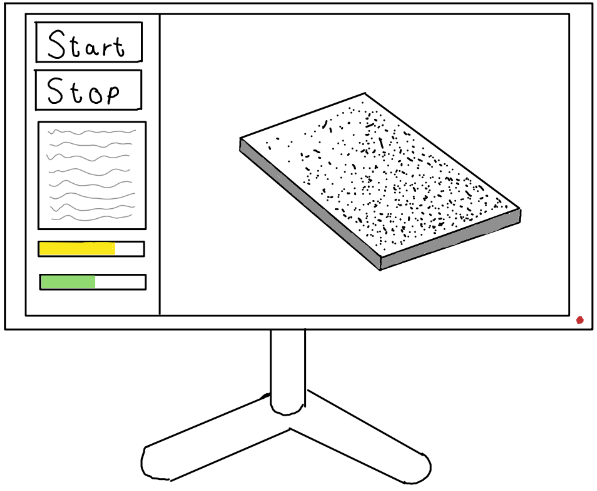
\includegraphics[width=0.80\linewidth]{Sections/5 Konceptgenerering/Media/Computer.png} & 
        
\includegraphics[width=0.80\linewidth]{Sections/5 Konceptgenerering/Media/Kamera.png} \\ \hline
        
        \rowcolor{aaublue}\multicolumn{7}{|c|}{\textcolor{white}{\textbf{Endelig koncept}}} \\ \hline
        \multicolumn{7}{|c|}{\includegraphics[width=0.80\linewidth]{Sections/5 Konceptgenerering/Media/Endelige løsning.png}} \\ \hline
    \end{tabularx}
\end{figure}
  
\end{comment}


\plainbreak{2}
\input{Sections/5 Konceptgenerering/5 Løsningsanalyse}
\subsection{Prikdosering} \label{Prikplacering}
Der er i den morfologiske analyse fundet frem til, at prikkerne påføres emnet med en mekanisme der doserer en dråbe. Dette sker uden kontakt til emnet, og der vælges at gøre brug af en eksisterende løsning, der implementeres i robotten. Af eksisterende metoder til præcis dosering af dråber er følgende; Piezoelectric Jet Valves (PeJV), Piezoeletric Pump (PeP) og Thermal InkJet (TIJ) udvalgt. 

%De 3 metoder undersøges, hvorefter en udvælges. 

%Ud fra vurderingen i \ref{Mekanisk system - vurdering} skal der udvikles en løsningen hvor "farven", påføres materialet uden kontakt. Der vil i det følgdene undersøges løsning muligheder, til at opnå prikplacering. Dette vælges som det første, for at lave overslags bergninger på stellets styrke. 


\textbf{Piezoelectric Jet Valves (PeJV)} fungere ved at en piezoelektrisk aktuator, flytter et stempel op og ned. Når stemplet flyttes op, kan væske bevæge sig ind i dyse hovedet. I det stemplet sænkes igen, vil stemplets kontakt med dyse hovedet, gør at væsken skydes ud af dysen, som vist i figur \ref{fig:PeJV}.

\begin{figure}[H]
    \centering
    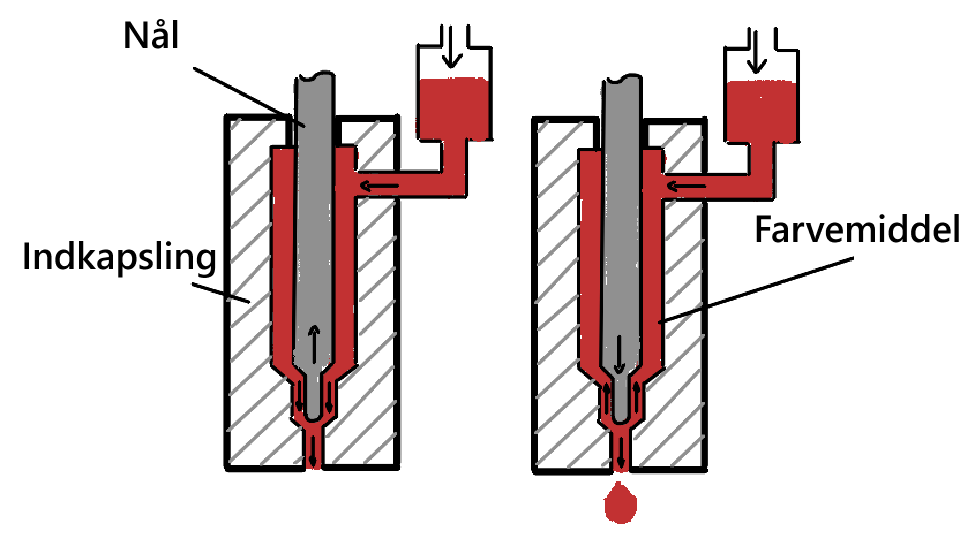
\includegraphics[width=0.6\linewidth]{Sections/5 Konceptgenerering/Media/PEJV.png}
    \caption{Ilustration af piezoelektrisk aktuator}
    \label{fig:PeJV}
\end{figure} \plainbreak{-.5}

 Processen gentages for hver gang der skal sættes en prik. Brugen af piezoelektrisk aktuator, betyder der er en høj kontrol af stemplets bevægelse, hvilket medfører en høj væske doseringspræcision, helt ned til \(\SI{0,5}{nL}\). Yderligere betyder brugen af piezoelektrisk aktuator, at cyklussen kan udføres med op til \(\SI{3000}{Hz}\). (\cite{VIEWEG2025JetDV-6210}; \cite{Hoath2016FundamentalsDroplets})


\plainbreak{1}
\textbf{Piezoeletric Pump (PeP)} bruger en piezoelektrisk aktuator til at danne et undertryk, som åbner indgangen til et kammer og trækker farve ind i kammeret. Dette fremgår af figur \ref{fig:PeMP}. Når kammeret er fyldt op bruges den piezoelektriske aktuator til at skabe et overtryk, der åbner udgangen og skubber farven ud. Ved PeP skubbes farven ud af et tryk, i modsætning til at blive skudt ud som ved PeJV. Dette resulterer i et simplere system, med et begrænset antal dele der bevæges. (\cite{Benaissa2012PerformancesPiezo-pump}; \cite{Hoath2016FundamentalsDroplets})

\begin{figure}[H]
    \centering
    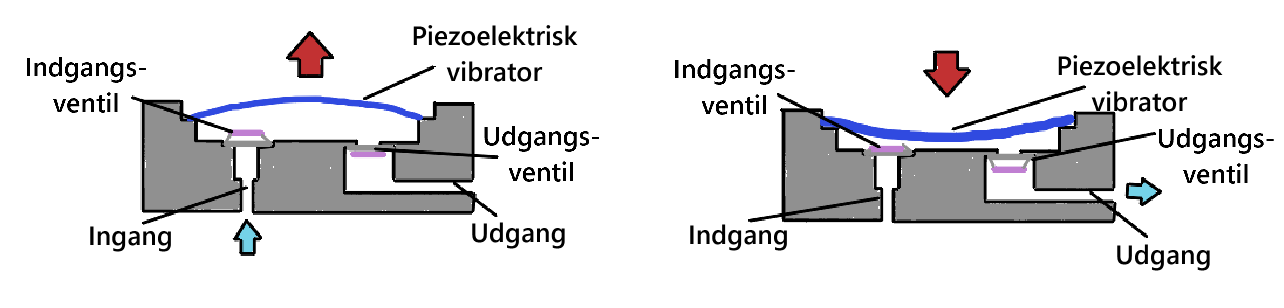
\includegraphics[width=1\linewidth]{Sections/5 Konceptgenerering/Media/pumpe.png}
    \caption{Illustration af piezoelektrisk pumpe}
    \label{fig:PeMP}
\end{figure} \plainbreak{-0.5}

PeP bruges ofte til at pumpe en væske kontinuerligt, hvilket betyder der ikke er gode muligheder for udføre doseringer, der kræver pauser imellem. Dette betyder for at gøre brug af PeP, skal der gøres brug af en kontinuerligt væskebevægelse, hvortil et andet system skal opsamle væsken der ikke skal doseres. Sådan et system introducerer kompleksitet tilbage i systemet.

\textbf{Thermal InkJet (TIJ)} fungerer ved, at blæk opvarmes indtil det fordamper og der opnås en indre boble i blækket. Den indre boble vil udøve et tryk på blækket, som vil medføre at blækket skubbes ud af en dyse. Når blækket er skubbet tilstrækkeligt ud af dysen, vil boblen kollapse, hvilket resultere i at der skabes et undertryk, der trækker nyt blæk ind til opvarmning, hvorefter processen gentages, dette illustreres på figur \ref{fig:TIJ figur}. 
Ved at gøre brug af opvarmning, har TIJ en begrænsning i forhold til hvor hurtigt der kan printes, da nye bobler først kan dannes efter forrige boble har forladt dysen. \parencite{Hoath2016FundamentalsDroplets}


\begin{figure}[H]
    \centering
    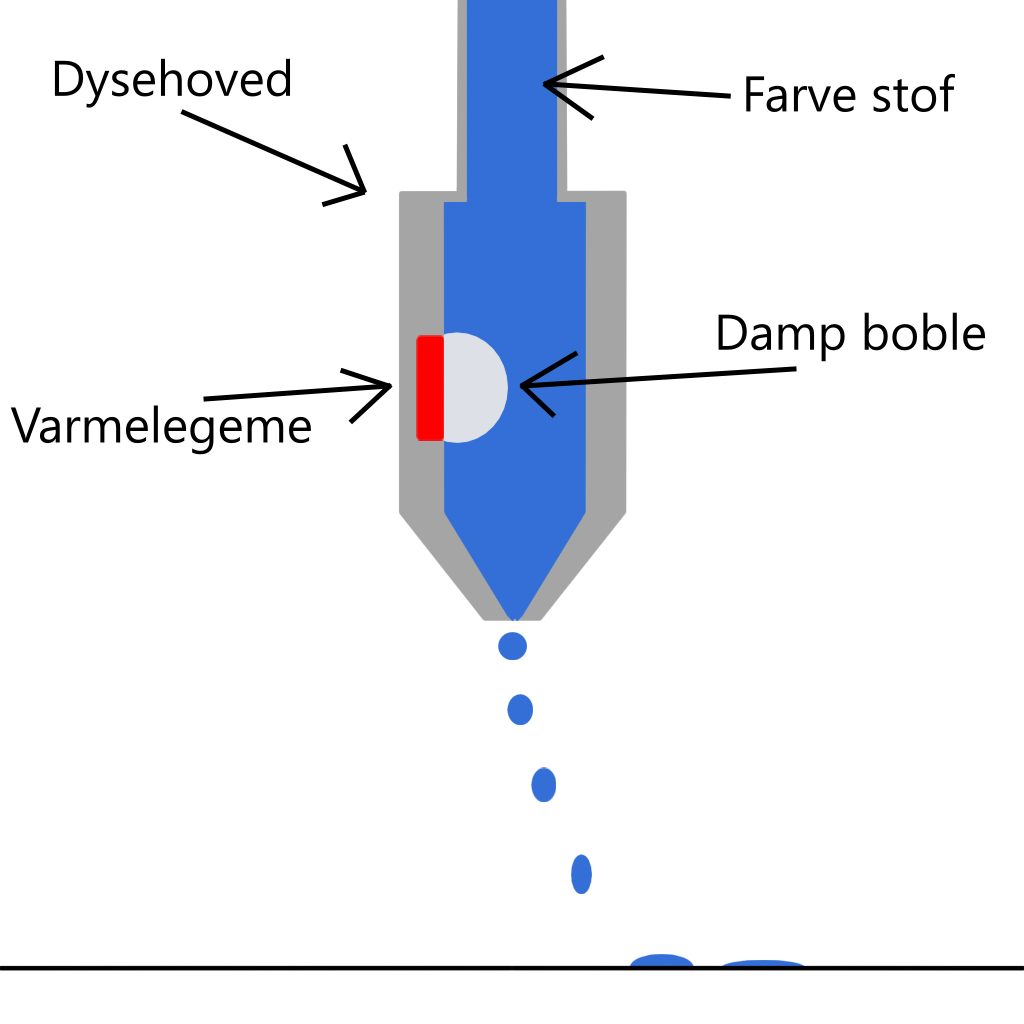
\includegraphics[width=0.35\linewidth]{Sections/6 Detaljeløsning/Media/TIJ figur 2.png}
    \caption{Illustration af thermal injekt teknik.}
    \label{fig:TIJ figur}
\end{figure} \plainbreak{-.5}

\subsubsection{Valg af doserings metode}  \plainbreak{-.5}
Det vælges at der anvendes en PeJV, fordi den kombinerer høj nøjagtighed, med høj gentagelseshastighed (op imod flere tusinde dråber i sekundet) uden at belaste farvestoffet med varme, hvilket sikre ensartede prikker i den ønskede størrelse. Samtidigt kræver PeJV ikke konstant flow og opsamling af overskydende væske, og den kan producere prikker i et bredt spænd. Alle disse egenskaber understøtter direkte de fremsatte krav omkring nøjagtighed, hastighed og fleksibilitet i løsningen. 

\plainbreak{2}
\subsection{Lineær bevægelse} \label{løsningsanal: Lineær bevægelse}
Det ønskes at finde en optimal bevægelsesform til flytning af prikemnet under prikpåføring. Fra designspecifikationer kan det ses, at der lægges vægt på præcision og hastighed af prikplacering. Dette vil bruges til at vægte forskellige lineære løsningsforslag, og vurdere den bedste løsning.
Af disse grunde, vælges der at udelukke løsninger der er upræcise, langsomme og evt. for komplicerede til at være en optimal løsning, dette efterlader valget mellem et tandremdrevet og et skruedrevet system. \parencite{IndustrialQuickSearch2025LinearPrinciples}

\textbf{Skruedrevet system} omfatter de to mest udbredte metoder; kugleskruer og ledeskruer. Ledeskruer omdanner roterende bevægelse til lineær bevægelse, gennem et gevind på skruen, hvortil genstanden der skal flyttes sidder på skruen se figur \ref{fig:Ledeskrue - skitse}. Ved at bevæge gevindet vil genstanden bevæge sig med gevindets spiral og derved bevæge sig frem ad.

Ledeskruer kræver færre dele og mindre vedligeholdelse end en kugleskrue. Tilgengæld er den mindre effektiv, grundet en større kontaktflade. Generelt gør ledeskruers simplere design, som ses i figur \ref{fig:Ledeskrue - skitse}, den billigere, men en kugleskrue kan have højere nøjagtighed og flytte tungere laster. Kugleskruers primære fordel er den lavere friktion og dermed højere effektivitet. Her er effektivitet et udtryk for forholdet mellem overført kraft og energi tabt til varme. (\cite{UniversalThreadGrindingCompany2020PrecisionAssemblies}; \cite{IndustrialQuickSearch2025LeadBenefits})

\begin{figure}[H]
    \centering
    \begin{subfigure}[b]{0.49\textwidth}
    \centering
        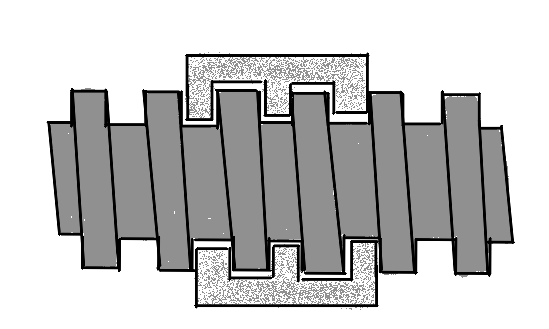
\includegraphics[width=\linewidth]{Sections/5 Konceptgenerering/Media/Ledeskrue-skitse.png}
      \caption{Skitse af ledeskrue}
       \label{fig:Ledeskrue - skitse} % Viljams mor når mig når(s)
  \end{subfigure}
    \hfill
  \begin{subfigure}[b]{0.49\textwidth}
    \centering
    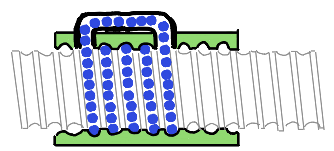
\includegraphics[width=\linewidth]{Sections/6 Detaljeløsning/Media/Ball nut.png}
    \caption{Kugleskrue illustration}
    \label{fig: Balls nut} % Mig når mig når når mig når viljams mor
  \end{subfigure}
    \caption{}
\end{figure} \plainbreak{-0.5}

Kugleskruer omsætter rotations kraft til lineære kraft, denne transformation opnås ved at rotere en skrue, hvorpå en kuglemøtrik er monteret. Kuglemøtriken indholder en mængde kugler, som bevæger sig i skurens gevind. Kuglernes bevægelse i gevindet resultere i at kuglemøtriken skubbes langs skruen. Kuglemøtrikens udformning muliggøre at kuglerne kan genanvendes, ved at når de når enden føres de gennem kuglemøtriken tilbage til fronten af kuglerækken (Se figur \ref{fig: Balls nut}). Kugleskruer har en højere effektivitet end ledeskruer, da rullende kugler har en lavere friktions koeficient end to flader, der gnider mod hinanden, som i en ledeskrue. Kugleskruers afvigelse ligger lidt under $\SI{0,0001}{mm}$. (\cite{Jaffe2025PrecisionGround}; \cite{IndustrialQuickSearch2025BallBenefits})


\textbf{Tandremsdrevede systemer} er kendetegnet ved, at en motor roterer en tandremskive hvorpå tandremmer sidder. Denne tandrem er koblet til en genstand, der ønskes at bevæges langs bæltets længde. Når tandremmen roteres den ene vej, vil emnet blive trukket i den retning, og modsatte retning hvis rotationsvejen vendes. Det tandremsdrevede system, er effektivt under lange arbejdslængder, og kan opnå store hastigheder. Tandremmene har en risiko for at glide, samt består af mere elastiske materialer end skruerne, hvilket kan medføre en afvigelse i præcision. Tandremmes afvigelse ligger omkring \(\SI{0,001}{mm/mm}\) \parencite{Rollco2022BallWhat}. 

\begin{figure}[H]
    \centering
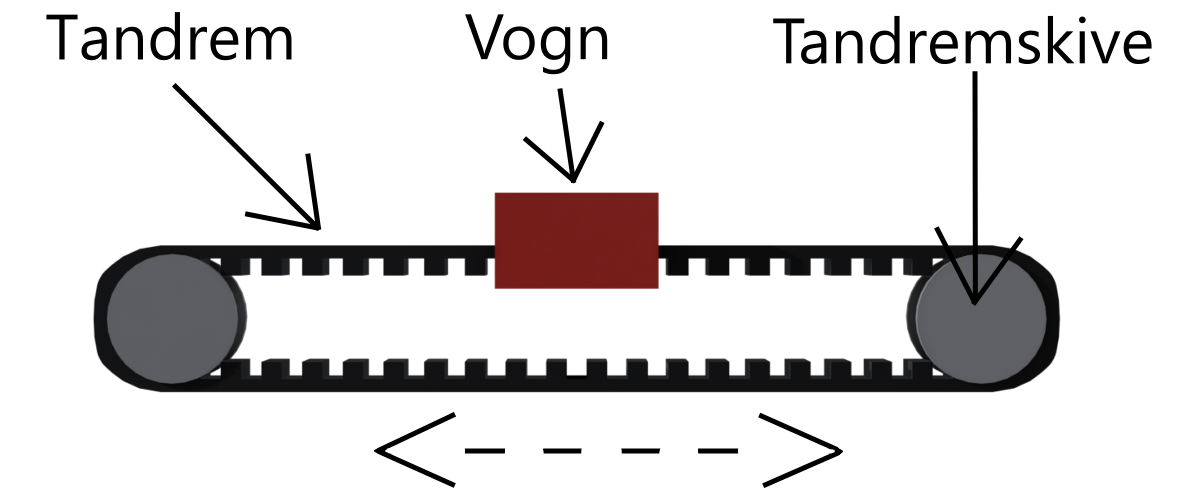
\includegraphics[width=0.6\linewidth]{Sections/5 Konceptgenerering/Media/Illustration af tandrem 7.png}
    \caption{Illustration af tandrem.}
    \label{fig: Illustration af tandrem}
\end{figure} \plainbreak{-.5}

Grundet materialerne tandremmen er lavet af varierer, sammen med remmene bliver svage i løbet af deres levetid, betyder dette at præcisionen af tandremme afhænger af mange faktorer. For at tandremssystemer kan opnå den nødvendige præcision, kræver det mere justering og er mindre pålideligt over løsningens levetid. \parencite{Casillo2025Belt-DrivenInc} 


\subsubsection{Valg af lineær bevægelse}  \plainbreak{-0.5}
Af forrige fremlagte muligheder, er kun ledeskruer og kugleskruer interessante, da der her skal fokuseres på korte afstande og stor præcision. Lede- og kugleskruer ligger begge mere end 1/5 under den maksimal acceptabel afvigelse på \(\SI{\pm0,1}{mm}\) over \(\SI{200}{mm}\), som er den største værdi i arbejdsområdets grænseværdi, hvilket gør begge brugbare.

Under prikplacering vil der ske mange accelerationer før arbejdsområdet er udfyldt, når der skiftes retninger. Dette betyder at en større acceleration vil gøre prikprocessen kortere. Accelerationen er en konsekvens af effektiviteten af skruen. Ledeskruer har typisk mellem 50\% og 70\% effektivitet, hvorimod kugleskuer har typisk over 90\% effektivitet. \parencite{johoty.com2025BallBest}

En ledeskrue bliver valgt til den lineære bevægelse, på trods af en lavere mekanisk effektivitet sammenlignet med en kugleskrue. Ledeskruer leverer den nødvendige præcision ($\approx \SI{d-4}{mm/mm}$) over kortere længder, og samtidigt kræver færre komponenter og minimal vedligeholdelse i forhold til kugleskruer. Deres simple design betyder også lavere materialeforbrug, samt færre dele at udskifte i tilfælde af nedbrud. 
\plainbreak{2}
\subsection{Endeligt koncept} \label{Endeligt koncept}
Det endelige konceptdesign fremgår af figur \ref{fig:skitse af endeligt koncept med navne}, hvor tre sæt af ledeskruer og følgestænger, danner bevægelsessystemet i henholdsvist to x-akser og én y akse.

\begin{figure}[H]
    \centering
    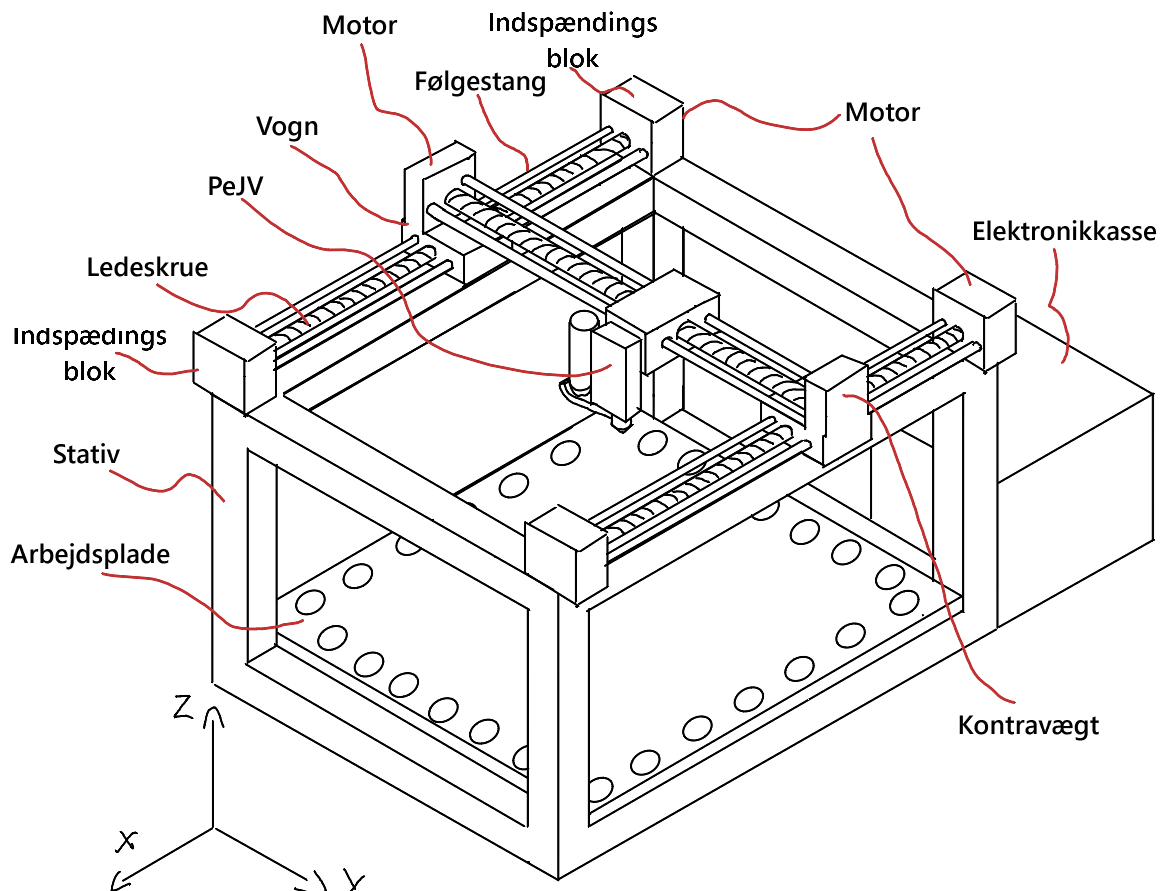
\includegraphics[width=0.7\linewidth]{Sections/6 Detaljeløsning/Media/Skitse med navne.png}
    \caption{Skitse af endeligt koncept med navne}
    \label{fig:skitse af endeligt koncept med navne}
\end{figure} \plainbreak{-.5}

Opsætningen er valgt med fokus på at sikre præcis lineær bevægelse af PeJV'en hen over emnet. I figuren ses, hvordan hovedet bevæger sig langs to parallelle følgestænger, hvor ledeskruen står for fremdriften. Denne mekaniske opsætning gør systemet stabilt, hvilket er nødvendigt for at opnå den påkrævede præcision.


